\section*{Prototype and Method}

The prototype was implemented in Unity as a sparse VR environment with a single target wall. The participant stands in front of the wall and completes measurement and exposure blocks without walking or changing room layout. This keeps the spatial frame stable while the current task and perturbation change. The system supports two input modes: controller-based pointing and embodied hand-tracking-based pointing. In both modes, the dominant hand is used for aiming and the non-dominant-hand controller trigger is used for confirmation. This opposite-hand confirmation was chosen to mitigate the Heisenberg effect of spatial interaction, where confirming a selection can perturb the tracked input pose and introduce selection-induced error \cite{wolf2020understanding}. It also kept confirmation comparable between input modes.

The runtime is organized around a central orchestration script, \texttt{SandboxRunner.cs}. It handles calibration, input abstraction, effect selection, confirmation, block progression, and logging hooks. A separate effect layer, \texttt{PrismCore.cs}, supplies the active translation, rotation, or skew transform. Task scripts then consume the unified input rather than implementing separate controller and hand-tracking pipelines. This structure was important because the prototype compares conditions; if each task handled input and effects independently, differences between conditions could be caused by implementation drift rather than the tested perturbation.

Figure~\ref{fig:article-prototype-view} illustrates the participant-facing environment that this runtime structure produces. The figure shows the shared target-wall setup and the embodied input view, making the stable room layout and reusable loading/progress cue visible before the individual perturbations are introduced.

\begin{figure*}[t]
    \centering
    \begin{minipage}[t]{0.49\linewidth}
        \centering
        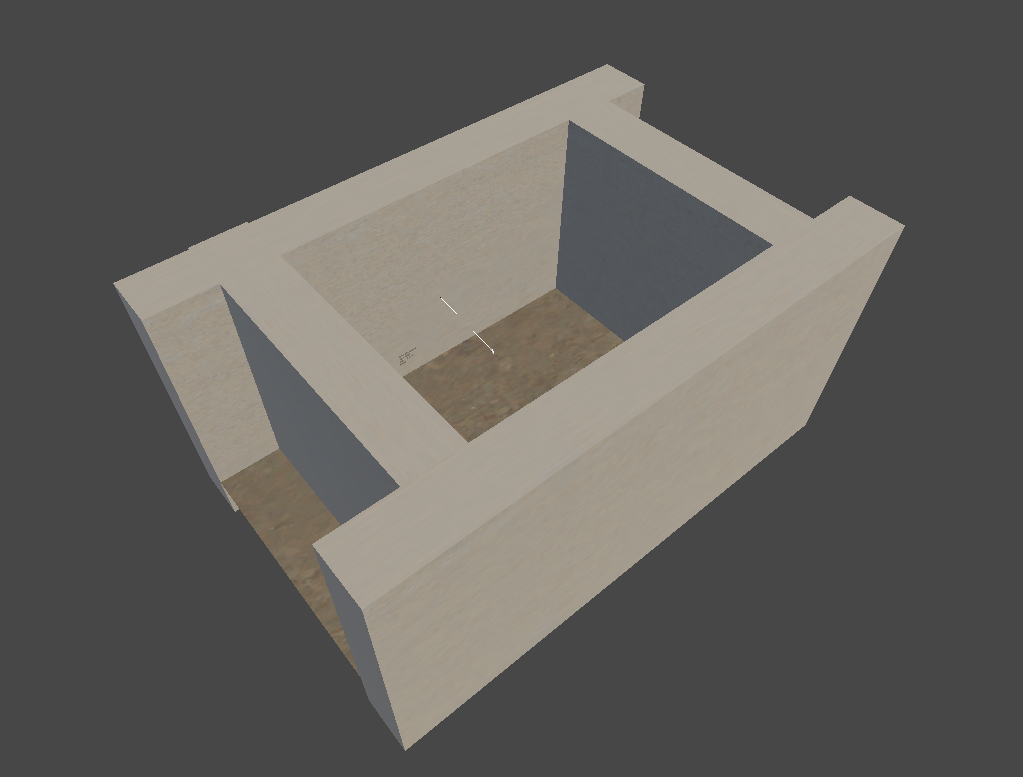
\includegraphics[width=\linewidth]{img/3_Implementation/FullView.png}
        \textbf{(a)} Shared VR scene
    \end{minipage}
    \hfill
    \begin{minipage}[t]{0.49\linewidth}
        \centering
        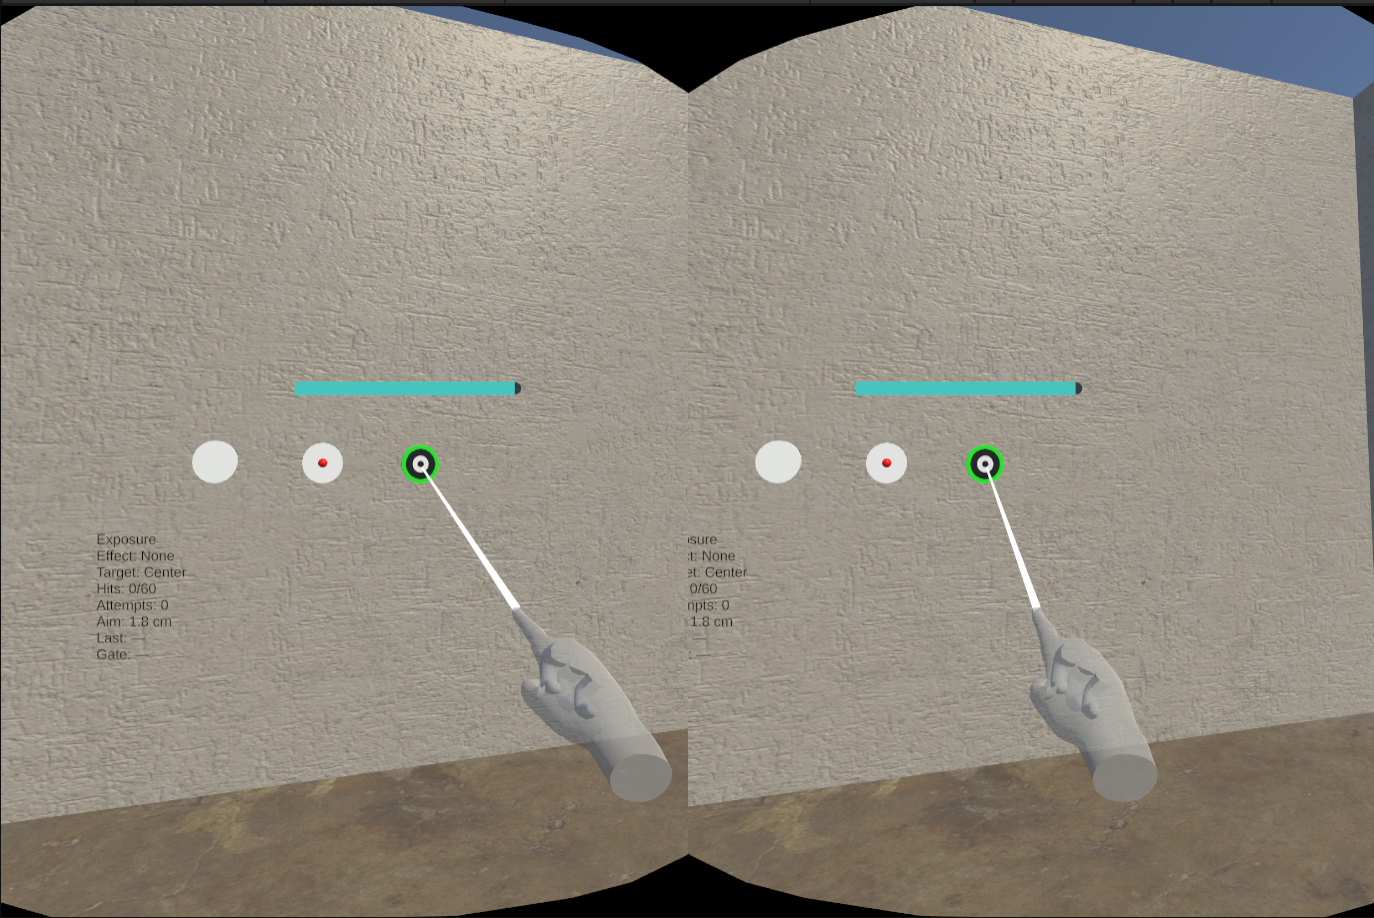
\includegraphics[width=\linewidth]{img/3_Implementation/EmbodyDefaultWithLoading.png}
        \textbf{(b)} Embodied input and progress cue
    \end{minipage}
    \caption{The prototype uses one sparse target-wall environment across tasks. The same wall, pointing representation, and loading/progress cue are reused so task and perturbation changes remain explicit.}
    \label{fig:article-prototype-view}
\end{figure*}

The implemented tasks follow a baseline--exposure--post structure. Open-loop pointing measures signed endpoint error relative to a point target. Line bisection measures signed deviation from the true midpoint of a horizontal line. Exposure uses a fixed horizontal three-target layout in which one target is active at a time. During exposure, the active perturbation is applied and each confirmed attempt is logged as a hit or miss. The prototype also implements a landmark task, but the final healthy-participant evaluation focused on open-loop pointing and line bisection.

The three active perturbation implementations are shown in Figure~\ref{fig:article-effect-views}. The figure uses the same exposure task in each panel, so the visual difference between translation, rotation, and skew can be compared without changing the task context.

\begin{figure*}[t]
    \centering
    \begin{minipage}[t]{0.32\linewidth}
        \centering
        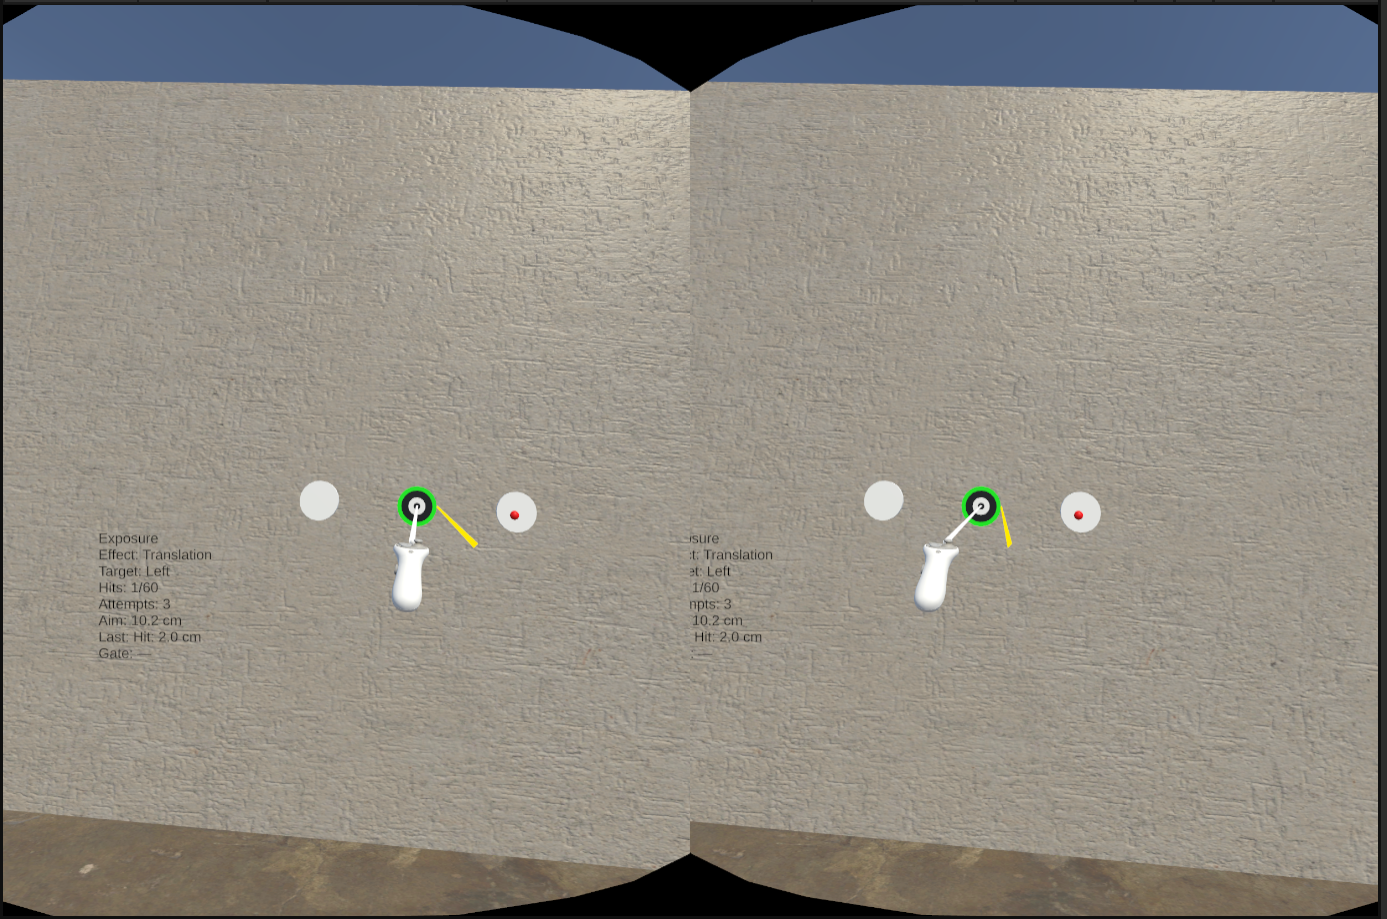
\includegraphics[width=\linewidth]{img/3_Implementation/ExposureTranslation1.png}
        \textbf{(a)} Translation
    \end{minipage}
    \hfill
    \begin{minipage}[t]{0.32\linewidth}
        \centering
        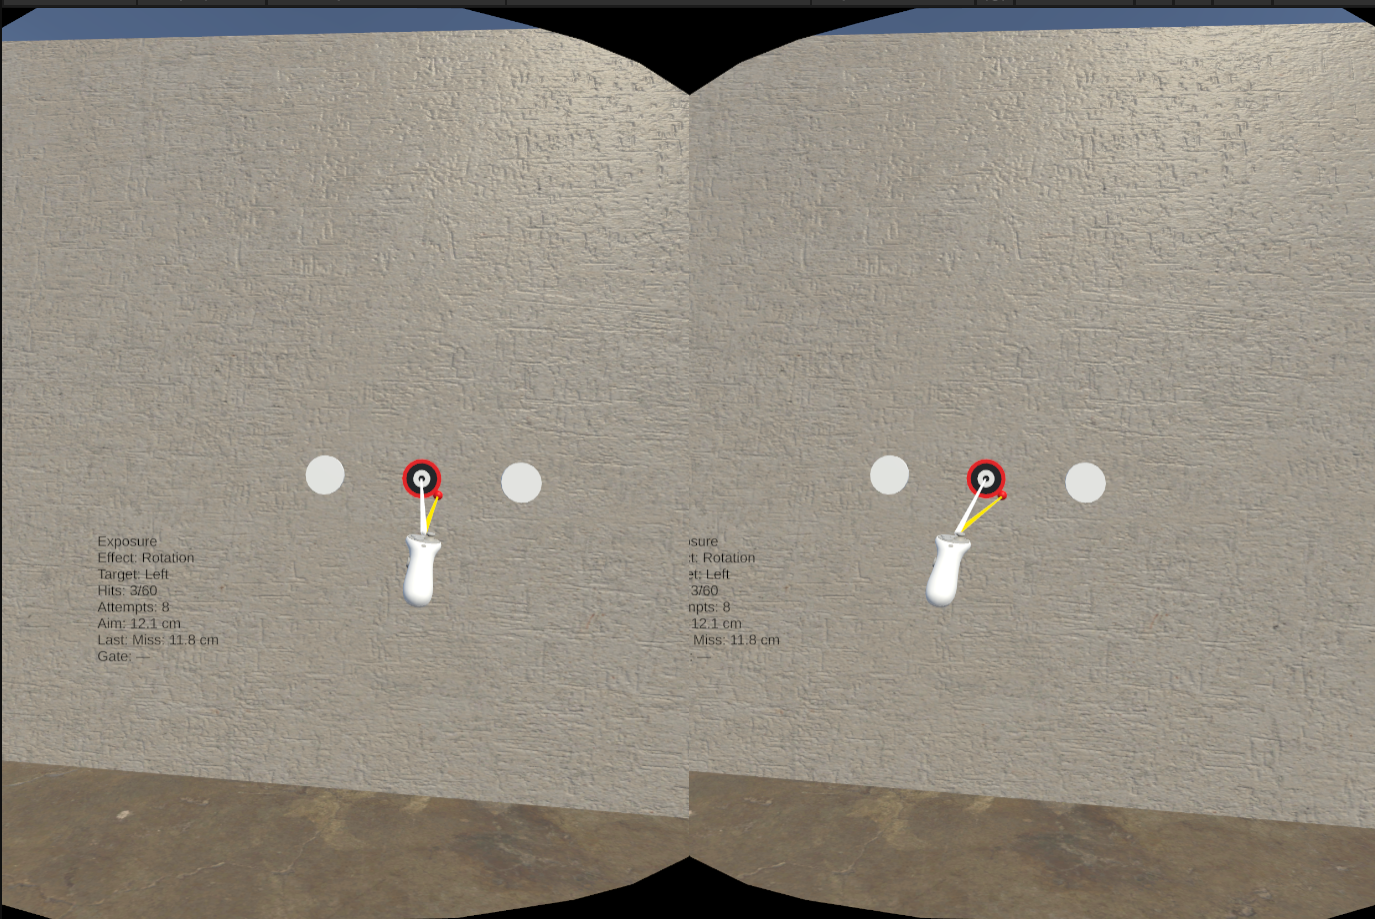
\includegraphics[width=\linewidth]{img/3_Implementation/ExposureRotate.png}
        \textbf{(b)} Rotation
    \end{minipage}
    \hfill
    \begin{minipage}[t]{0.32\linewidth}
        \centering
        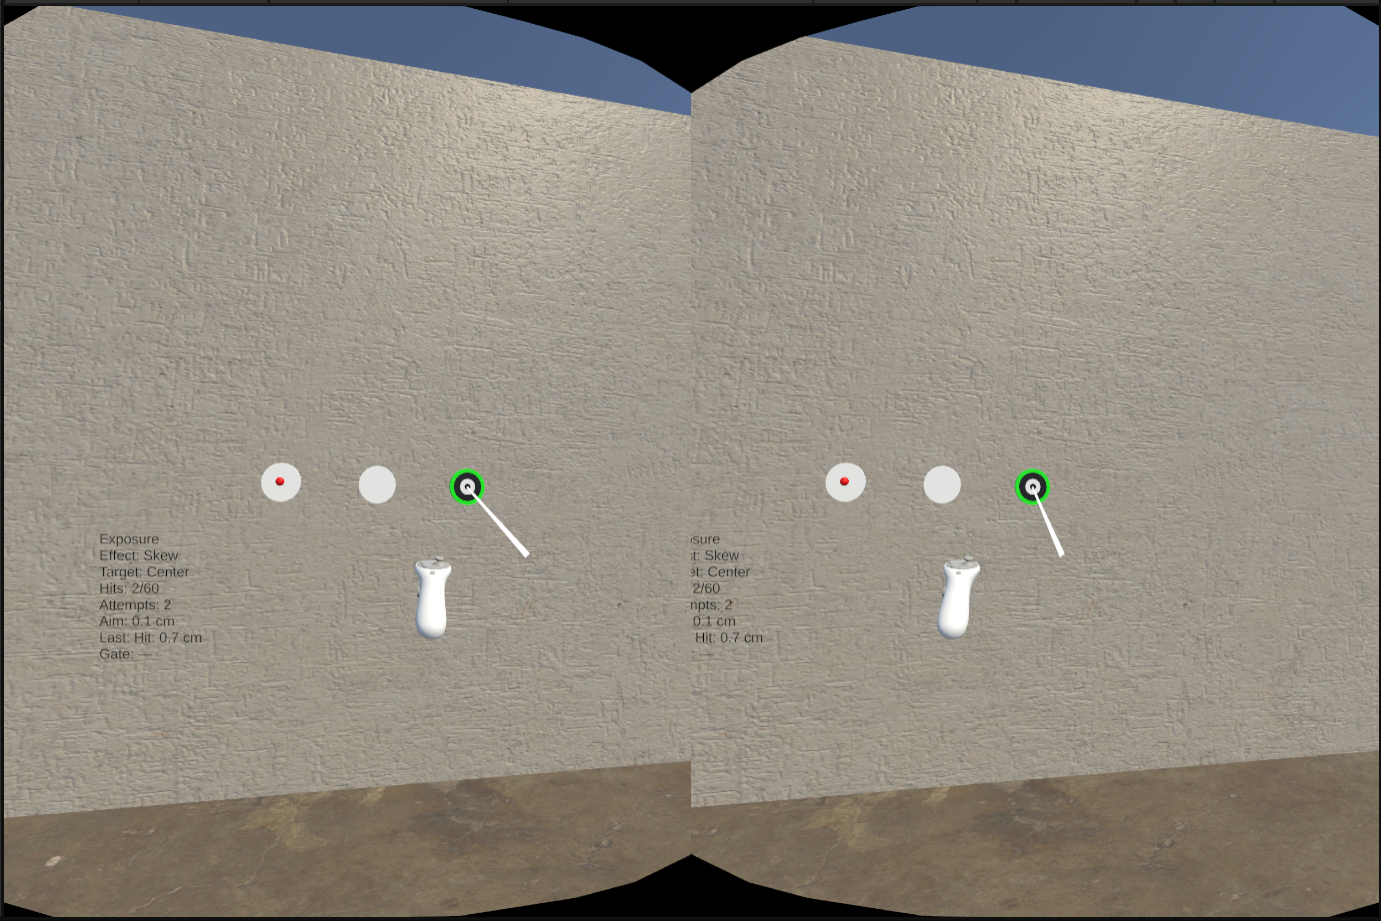
\includegraphics[width=\linewidth]{img/3_Implementation/ExposureSkew.png}
        \textbf{(c)} Skew
    \end{minipage}
    \caption{The same exposure task under three perturbation implementations. Translation shifts the response origin, rotation changes the pointing direction, and skew shifts the visible pointing representation together with its corresponding aim.}
    \label{fig:article-effect-views}
\end{figure*}

The logging layer writes four CSV collections per module: metadata, discrete events, continuous samples, and summary rows. These are loaded by an RShiny dashboard with views for single-session summaries, cross-session comparison, participant-level profiles, exposure quality, spatial landing patterns, and movement trajectories. The analysis therefore does not depend only on one after-effect number; it also allows each module to be checked for rushed exposure, low hit rate, tracking problems, spatial spread, or unusual trajectory behaviour.
